% Mechanical Systems and Signal Processing -- research paper.
% Compile: pdflatex main; bibtex main; pdflatex main; pdflatex main   (elsarticle + elsarticle-num)
% Every table in tables/ is generated by paper/make_tables.py; every figure by a script in paper/figures/.
\documentclass[preprint,3p,times]{elsarticle}

\usepackage{amsmath,amssymb}
\usepackage{booktabs}
\usepackage{graphicx}
\usepackage[table]{xcolor}
\usepackage{url}
\usepackage[hidelinks]{hyperref}
\usepackage{siunitx}
\sisetup{detect-all,group-separator={,}}

\journal{Mechanical Systems and Signal Processing}

\begin{document}

\begin{frontmatter}

\title{Bearing leakage survives source-free adaptation: a bearing-wise evaluation of SDALR and SHOT with physics-gated pseudo-labels}

\author[a]{Mohammad Rafiur Rahman\corref{cor1}}
\ead{u2303064@student.cuet.ac.bd}
\cortext[cor1]{Corresponding author.}
\address[a]{Department of Mechanical Engineering, Chittagong University of Engineering \& Technology (CUET), Chattogram 4349, Bangladesh}

\begin{abstract}
Source-free domain adaptation (SFDA) reports near-ceiling accuracy for rolling-bearing diagnosis, but its protocols place
the same physical bearings on both sides of a transfer. We re-evaluate a published SFDA method (SDALR) and SHOT on the
Paderborn data in a paired design: one source model is adapted to the same bearings and to unseen bearings at the same
target condition. Over ten pre-registered bearing splits, unseen bearings cost a median 36.2 points (95\,\% CI 25.0--56.3,
10 of 10 splits), and a given bearing loses a median 38.7 points when it is unseen rather than seen. The gap is already
present before adaptation (35.1 points): neither method's adaptation creates or repairs it. SHOT, non-adaptive random
forests and a fixed-condition control show the same loss, and a second rig, where specimen and bearing size change together, shows a loss of similar direction and size. It is not a
fixed identity shortcut. In a random forest, accuracy on unseen
bearings rises from \SI{46}{\percent} to \SI{75}{\percent} as the source grows from one to four bearings per class, so
three specimens per class under-sample the damage signatures. An oracle pseudo-label filter recovers a median
\SI{82}{\percent} of the loss. Envelope-based kinematic gates accept 0 to 9 of 480 healthy recordings as faulty, against
214 for a raw-spectrum band rule, but certify only the specimens with the largest damage. Inside the adaptation loop the
safe gate adds a median 4.5 points, almost all of it on the recordings it certifies. We list the evidence such results
should carry.

\end{abstract}

\begin{highlights}
\item Unseen bearings cut SDALR accuracy by a median 36 points and SHOT accuracy by 22.
\item The gap exists before adaptation; SDALR and SHOT neither create nor repair it.
\item On unseen bearings a forest scores 46\% with 1 source bearing per class, 75\% with 4.
\item Envelope gates are safe on healthy bearings but certify only the largest damages.
\item A pseudo-label oracle and a shallow baseline belong in every SFDA comparison.
\end{highlights}

\begin{keyword}
rolling bearing \sep source-free domain adaptation \sep data leakage \sep bearing-wise evaluation \sep
pseudo-label gating \sep envelope analysis
\end{keyword}

\end{frontmatter}

\section{Introduction}
\label{sec:intro}

Rolling-element bearings fail in service, and the vibration signature of a spall or a crack is well understood: an impact
train at a kinematic frequency fixed by the bearing geometry and the shaft speed, modulated by load and smeared by cage slip
\cite{randall2011}. Condition-monitoring practice turns that signature into a decision --- replace the bearing, or leave it
--- and the value of an automated diagnosis is the reliability of that decision on a bearing the diagnostic system has not
seen before.

Data-driven diagnosis has moved towards transfer learning to meet that requirement. Unsupervised domain adaptation
transfers a model trained under one operating condition to another without target labels \cite{zhao2021udtl}, and source-free
domain adaptation (SFDA) goes further: during adaptation only the trained source model and unlabelled target recordings are
available, which suits an operator who cannot ship raw data between sites \cite{liang2020shot,sdalr2025}. Reported
accuracies are high. Vieira et al.\ sampled 18 supervised bearing-diagnosis papers published in 2025: every one reported
above \SI{94}{\percent}, five reported \SI{100}{\percent}, and none split training and test data by physical bearing ---
eight split at random, nine by condition (load, speed or noise level) and one did not state its split
\cite[Table~1]{vieira2026}. Source-free results sit at the same level: the method we re-evaluate, SDALR, reports
\SI{96.8}{\percent} on Paderborn \cite{sdalr2025} on a task whose eight classes are eight individual bearings, the same
specimens on the source and the target side.

A vibration dataset carries two kinds of information at once. One is the fault physics that should transfer: the impact
train at the outer-race or inner-race passing frequency. The other is everything particular to one specimen --- the extent
and shape of its damage, its mechanism, its mounting, clearance and resonances. When the same physical bearing appears in
training and in test, the particulars are sufficient to score well, and no experiment in that protocol can tell the two
apart. Splitting by physical bearing removes the shortcut, and in supervised settings it has been shown to change
conclusions \cite{hendriks2022,wheat2024leakage,vieira2026,kaya2026}; the same lesson was learned in clinical machine
learning, where record-wise rather than subject-wise splits overestimate accuracy \cite{saeb2017}.

SFDA deserves separate scrutiny for a reason specific to how it works. Adaptation is driven by the source model's own
predictions on target data --- pseudo-labels, centroids or neighbourhood structure --- refined over iterations. If the
source model has learned the particulars of its training specimens, adaptation might sharpen that error on a new bearing,
or it might repair it. Which one happens, how much performance is at stake, and what physics-based pseudo-label filters can
recover are empirical questions that a leaky protocol cannot ask. Physics-based filters are increasingly proposed:
characteristic-frequency evidence gates and weights pseudo-labels in the EAGLE module of Bio-SFDA \cite{yoon2026biosfda}
and builds physical pseudo-labels in PIUDA \cite{jia2024piuda}, and a physics consistency validator supervises confidence
in PCTL \cite{pctl2026}. These modules are judged by end accuracy; how often they declare a fault on a healthy bearing ---
which decides whether they are safe inside an adaptation loop --- is not reported in those works.

This paper follows one thread through those questions, with every decision rule fixed in a versioned protocol before the
corresponding run.

\begin{enumerate}
  \item \textbf{How much survives, and where the loss arises.} One source model is adapted to the same bearings and to
        unseen bearings at the same target condition (Section~\ref{sec:protocol}). We measure the gap on ten
        pre-registered random bearing splits, two mechanical folds and a second rig, for two SFDA methods and for
        non-adaptive baselines, before and after adaptation, and for each bearing when it is seen and when it is unseen
        (Sections~\ref{sec:res-collapse} and~\ref{sec:res-second}).
  \item \textbf{Why unseen bearings fail.} Probes, a per-bearing table drawn from the dataset's own damage profiles and a
        pre-registered source-diversity curve separate a fixed identity shortcut from under-sampled damage signatures;
        a classifier on kinematic envelope features tests whether the loss is specific to the input representation
        (Section~\ref{sec:res-mechanism}).
  \item \textbf{What any pseudo-label filter could recover.} An oracle filter that keeps only correct pseudo-labels gives a
        reference for keep-or-withhold filters (Section~\ref{sec:res-decomp}).
  \item \textbf{What physics gating actually buys.} Four gates are compared by false acceptance on 480 real healthy
        recordings and over their full operating curves, then inserted into the adaptation loop as paired arms
        (Section~\ref{sec:res-gating}).
\end{enumerate}

The novelty is narrow, and we state it against the nearest work. That bearing overlap inflates diagnosis accuracy is
established: Hendriks et al.\ on CWRU \cite{hendriks2022}, Wheat et al.\ across run, day and part splits
\cite{wheat2024leakage}, and Vieira et al., who also hold the training set fixed and change only the test set, including a
same-bearing, same-condition repetition-wise split on Paderborn \cite[Section~6.2]{vieira2026}. Knap et al.\ built a
recording-separated cross-domain benchmark with one cross-bearing scenario \cite{knap2026leakagesafe}, and concurrent
work adapts across Paderborn conditions with held-out bearings, without a leaky baseline or a source-free method
\cite{nagaswetha2026}. All of these are supervised, non-adaptive or source-dependent. What this paper adds is (i) the
fixed-source design applied to SFDA, with a source-only arm that locates the loss before adaptation and a within-bearing
contrast that holds the specimen fixed; (ii) a pre-registered source-diversity curve and a kinematic-feature control that
bear on why unseen bearings fail; (iii) the perfect-pseudo-label reference of Schlachter et al.\ \cite{schlachter2025},
applied as a keep-or-withhold oracle and set against the loss; and (iv) false-acceptance curves on real healthy recordings
for the physics gates that such methods insert, with the gates' coverage traced to the size of each specimen's damage.

We claim no new network, detector or adaptation algorithm. Statistical envelope thresholds are established
\cite{borghesani2013,randall2011} and harmonic-coordinate features close to the ones used here were published by Matania et
al.\ \cite{matania2025}. The contribution is knowledge about where the error of source-free bearing diagnosis lies, what
physics-based filtering can and cannot repair, and the evidence a result in this area should carry before it is believed.

\section{Background and related work}
\label{sec:background}

\subsection{Leakage in bearing-diagnosis evaluation}

Hendriks, Dumond and Knox showed that the conventional condition-wise split of the CWRU data places the same physical
bearings in training and test sets, and proposed benchmarking with independent sets of bearings \cite{hendriks2022}. Wheat et
al.\ compared run-to-run, day-to-day and part-to-part splits for classical pipelines and found accuracy falling by more than
40\,\% between the most and least separated splits \cite{wheat2024leakage}. Vieira et al.\ generalised bearing-wise
partitioning, reformulated diagnosis as multi-label detection, and measured the inflation caused by segmentation-level and
bearing-level leakage on UORED, Paderborn and CWRU with the training set held fixed and only the test set changed
\cite{vieira2026}. On Paderborn their repetition-wise split --- training and test recordings from the same bearing at the
same condition --- scores near-perfect Macro-AUROC against 54--77\,\% without leakage \cite[Table~12]{vieira2026}. Their study
is supervised and, in their words, concerns ``training and testing within a single testbench''; it does not evaluate
adaptation. Matania et al.\ \cite{matania2024leakage} show how test--training separation should be constructed for bearing
fault classification. Knap et al.\ published a leakage-safe cross-domain benchmark on CWRU and Paderborn with six fixed
scenarios \cite{knap2026leakagesafe}; its default rule separates \emph{recordings}, and one scenario holds out bearings,
which they report among the hardest. Kaya and Jobani report a fall from about 0.86 to 0.56 macro-F1 when Paderborn
bearings are made disjoint in a supervised pipeline \cite{kaya2026}. Concurrently, Nagaswetha and Pathak adapt across
Paderborn conditions with held-out bearings and find that an order-domain representation decides whether alignment helps
\cite{nagaswetha2026}; they use source data and no leaky baseline.

Beyond this field, Kapoor and Narayanan document leakage across 17 scientific disciplines and give the taxonomy we adopt
\cite{kapoor2023leakage}, Saeb et al.\ show the record-wise versus subject-wise analogue in clinical prediction
\cite{saeb2017}, and Geirhos et al.\ name the learning behaviour at stake: a shortcut that succeeds on the benchmark and fails
under the intended shift \cite{geirhos2020shortcut}.

\subsection{Source-free domain adaptation for bearings}

SHOT established the template on which most later methods build: freeze the source classifier, maximise information at the
target and refine centroid-based pseudo-labels \cite{liang2020shot}. SDALR extends it by separating reliable from unreliable
target predictions, using the reliable ones as supervision and the unreliable ones through an entropy term, and reports
\SI{96.8}{\percent} mean accuracy across Paderborn operating conditions \cite{sdalr2025}. Its Paderborn task has eight
classes, each a single physical bearing (K001, KA04, KA15, KA22, KA30, KI14, KI17, KI21), and the same eight specimens form
the source and the target, so the reported transfer is between operating conditions of known bearings. Other source-free
work crosses rigs: Jeong et al.\ combine order normalisation with test-time training and evaluate on a test-only machine
\cite{jeong2025}, and Bio-SFDA reports a CWRU-to-Paderborn task \cite{yoon2026biosfda}. A cross-rig target is
bearing-disjoint by construction, but it changes rig, bearing type, sensor and often label space at once, so it cannot say
how much of the loss is the specimen. Neither design asks how a source-free method fares on unseen bearings of the rig it
was trained on, which is the question here.

\subsection{Physics priors inside adaptation}

Characteristic frequencies computed from geometry and speed are the natural prior for bearing diagnosis. PIUDA builds
physical labels from fault-characteristic spectral energy and aligns them into pseudo-labels for transfer between different machines
\cite{jia2024piuda}. Bio-SFDA gates and weights pseudo-labels with band-energy and signal-to-noise predicates at BPFO, BPFI
and BSF computed on a short-time Fourier transform, with thresholds rescaled online from unlabelled target statistics
\cite{yoon2026biosfda}. PCTL scores the envelope spectrum predicted from the model's features against characteristic
frequencies and uses that score to supervise a confidence predictor while fine-tuning on a small labelled target set
\cite{pctl2026}; it does not filter pseudo-labels. In none of these works is the rate at which the module accepts a fault on
a healthy bearing reported. Because the Bio-SFDA task definition for Paderborn cannot be reconstructed from the article --- a
ball class is listed although the Paderborn real-damage set contains no rolling-element damage --- we evaluate the gating
\emph{mechanism as described, as we implemented it}, and make no comparison against the accuracy reported there.
Schlachter et al.\ simulate pseudo-labelling with ground truth in source-free universal adaptation and report the upper
level that perfect pseudo-labels reach \cite{schlachter2025}; our oracle filter is the keep-or-withhold version of that
instrument.

\subsection{Envelope analysis and the statistics of detection}

The squared envelope spectrum is the standard carrier of second-order cyclostationary bearing signatures \cite{randall2011},
usually after a band selection such as the fast kurtogram \cite{antoni2007kurtogram} and, where discrete components
dominate, after discrete/random separation. Borghesani et al.\ derived the statistics of the squared envelope spectrum under
coloured noise and the corresponding thresholds for testing cyclostationarity \cite{borghesani2013}. The gates compared here
are built from those ingredients; none is claimed as new. Matania et al.\ project order-domain envelope spectra onto
kinematic positions to obtain a machine-invariant representation \cite{matania2025}, the same idea as the harmonic
coordinates used inside our comb tests and our kinematic-feature control.

\section{Test rigs, bearings and kinematics}
\label{sec:data}

\begin{table}[htbp]
\centering
\caption{Test rigs and recordings used in this study. Bearings are physical bearings, not fault classes.}
\label{tab:datasets}
\small
\setlength{\tabcolsep}{4pt}
\begin{tabular}{lllrrl}
\toprule
Dataset & Bearings used & $f_s$ (kHz) & Record (s) & Conditions & Role \\
\midrule
Paderborn (PU) \cite{lessmeier2016} & 6 healthy, 5 outer, 6 inner (real) & 64 & 4 & 4 (3 adapt.) & adaptation, gating, slip \\
HUST bearing \cite{thuan2023hust} & 5 types $\times$ \{healthy, inner, outer\} & 51.2 & 10 & 3 loads & second-rig replication \\
CWRU \cite{smith2015} & 6205 drive end, 6203 fan end & 12 / 48$^{a}$ & $\approx$10 & 4 loads & slip, contamination \\
UORED-VAFCLS \cite{sehri2023uored} & 20 bearings, natural faults & 42 & 10 & 1 & gate safety (suppl.) \\
JNU \cite{li2013jnu} & as published & 50 & 20 & 3 speeds & reproduction only \\
\bottomrule
\end{tabular}
\begin{minipage}{\linewidth}\vspace{2pt}\footnotesize $^{a}$ Fault recordings 12~kHz; the four normal baselines used for off-rig calibration 48~kHz. Paderborn: three conditions at 1500~rpm (25~Hz) for adaptation, all four for the gate and slip analyses. JNU: the three nominal speeds of the distributed data, as used by SDALR.\end{minipage}
\end{table}


Table~\ref{tab:datasets} lists the recordings used. \textbf{Paderborn} \cite{lessmeier2016} carries the adaptation
experiments: its 6 healthy bearings and the 5 outer-race and 6 inner-race bearings of its real-damage set, each recorded 20
times at four operating conditions, are the largest public combination we know of with several physical bearings per class
\emph{and} several operating conditions per bearing, which the paired design of Section~\ref{sec:protocol} needs. We use the
three conditions that share a nominal speed of \SI{1500}{rpm} (\SI{25}{Hz}) and differ in load and radial force, denoted A1
(N15\_M01\_F10), A2 (N15\_M07\_F04) and A3 (N15\_M07\_F10); the fourth condition (N09, \SI{900}{rpm}, \SI{15}{Hz}) enters
only the gate analyses.
\textbf{HUST bearing} \cite{thuan2023hust} provides the second-rig replication: one physical bearing per class for each of
five bearing types (6204--6208) at three motor loads, giving the same three-domain, six-task structure with the same label
space. \textbf{CWRU} \cite{smith2015} and \textbf{UORED-VAFCLS} \cite{sehri2023uored} appear only in the off-rig calibration of the
gate operating point and in the supplementary slip measurement. JNU \cite{li2013jnu} is used only to reproduce the published SDALR result.

Throughout, a \emph{bearing} means a physical specimen, identified by its dataset code (for example Paderborn KA04), not a
fault class or a damage severity. The label space is $\{\text{normal},\text{inner race},\text{outer race}\}$: Paderborn's
real-damage set contains no rolling-element damage, so a ball class cannot be formed from it, and HUST's ball recordings are
excluded for comparability.

\subsection{Kinematics are resolved per bearing}
\label{sec:kinematics}

Characteristic orders follow from the ball count $n$, ball diameter $d$, pitch diameter $D$ and contact angle $\theta$
through $r=(d/D)\cos\theta$, giving $\mathrm{BPFO}=\tfrac{n}{2}(1-r)$, $\mathrm{BPFI}=\tfrac{n}{2}(1+r)$ and
$\mathrm{FTF}=\tfrac{1}{2}(1-r)$ in shaft orders. A bearing designation does not determine these values. Paderborn's
per-bearing documentation, distributed with the data as one ``Profile of rolling bearing damage'' datasheet per specimen
rather than in the dataset paper, carries the geometry on page~1 of each file. Reading all 32 datasheets gives a clean
split by manufacturer: 26 specimens state ``Pitch circle diameter mm 29.05'' (IBU and MTK) and 6 state
\SI{28.55}{\milli\metre} (FAG), all with ``Number of rolling elements pc. 8'' and rolling elements of
\SI{6.75}{\milli\metre}. The 29.05 group contains every healthy specimen K001--K006 and the real-damage bearings KA16,
KA22, KA30, KI04, KI14, KI17 and KI18 (e.g.\ \texttt{data/pu/K001/K001.pdf}); the 28.55 group contains KA04, KA15, KI16
and KI21 (e.g.\ \texttt{data/pu/KA04/KA04.pdf}) together with KB24 and KB27, which this study excludes. Per-specimen
geometry and damage mode are listed in Supplementary~S3; the damage modes are used in Section~\ref{sec:limitations}. The corresponding
outer-race orders are 3.0706 and 3.0543, neither of which equals the 3.0531 of the CWRU SKF 6203 that is frequently reused
for Paderborn. We compute kinematics separately for each specimen, and no gate is computed for a bearing whose geometry its own rig does
not publish. HUST is such a case: its dataset paper gives bore, outside and ball diameters and the ball count, but not the
pitch diameter and no characteristic orders \cite{thuan2023hust}. Substituting the nominal mean diameter $(d_i+d_o)/2$
would supply the missing number, and it is worth seeing what that costs: on Paderborn, where the true value is documented,
the same substitution gives \SI{28.50}{\milli\metre} against \SI{29.05}{\milli\metre} and shifts the outer-race order by
\SI{0.58}{\percent}, a systematic error larger than the 5--95\,\% range of slip we measure on that geometry
(\SI{0.53}{\percent}, Supplementary~S5). The gate's $\pm\SI{2}{\percent}$ slip window would absorb such an error, but only by
spending its tolerance on a geometry guess rather than on slip, and a guessed geometry would make every HUST verdict
untraceable. We therefore use HUST for raw windows only and report no HUST gating result. Shaft speed is taken per
recording from the measured speed channel on Paderborn and from the in-file value on CWRU.

\subsection{What a window can represent}
\label{sec:windows}

The adaptation experiments use SDALR's input contract: windows of 2048 samples (Section~\ref{sec:protocol}). At
\SI{64}{kHz} and \SI{25}{Hz} shaft speed a window lasts \SI{32}{ms}, 0.8 shaft revolutions and about 2.5 outer-race
impacts; its envelope spectrum has a resolution of \SI{31}{Hz}, so the first outer-race (\SI{77}{Hz}) and inner-race
(\SI{123}{Hz}) lines lie about 1.5 bins apart. A window can carry the impulsiveness and energy of a fault but not its
kinematic signature. The gates, by contrast, use the first 249\,600 samples of each recording (\SI{3.9}{s}, resolution
\SI{0.26}{Hz}, about twelve bins inside the slip window of the first outer-race harmonic). Section~\ref{sec:res-mechanism}
tests what the difference is worth with a classifier built on the gates' representation.

\section{Evaluation protocol}
\label{sec:protocol}

\begin{figure}[htbp]
\centering
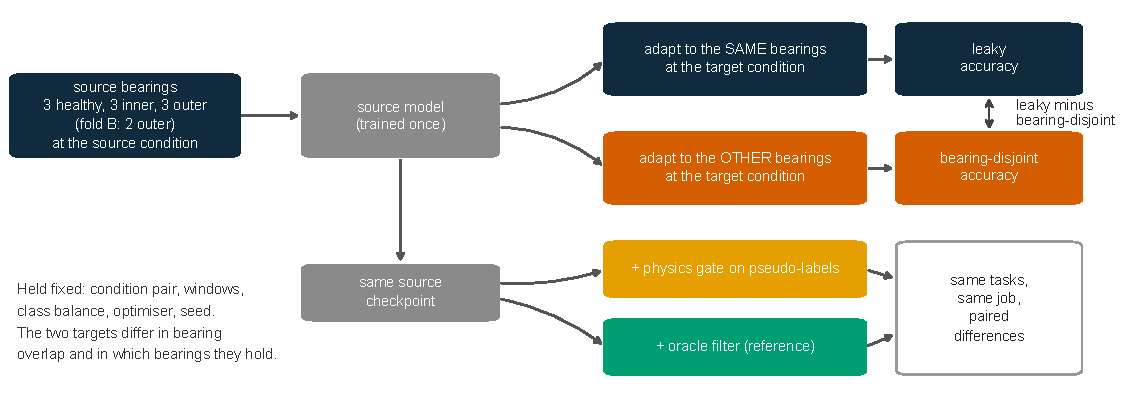
\includegraphics[width=\linewidth]{figures/fig1_design.pdf}
\caption{The paired design. One source model is trained on the source bearings at the source condition and then adapted
twice: to the \emph{same} bearings at the target condition (leaky) and to the complementary bearings at the same target
condition (bearing-disjoint, or clean). Both targets share the operating condition, the window contract and the class
balance. Gated and oracle arms reuse the same source checkpoint inside the same job, so their comparison with the ungated
clean arm is paired.}
\label{fig:design}
\end{figure}

\subsection{The paired leaky/clean design}

A source bearing set of 3 healthy, 3 outer-race and 3 inner-race specimens is trained at one operating condition. The
resulting source model is then adapted, without target labels, to two different targets at the same target condition
(Fig.~\ref{fig:design}): the \emph{leaky} target, made of the same physical bearings, and the \emph{clean} target, made of
the complementary bearings. Operating condition, window length, number of windows per class, class balance, optimiser,
schedule and seed are held fixed, as in the fixed-training designs of Vieira et al.\ \cite{vieira2026}. The leaky--clean
difference, written $\Delta_{\mathrm{leak}}$, therefore measures bearing overlap \emph{together with} the difference between
the two bearing sets, which hold different specimens. Two further contrasts separate these. The \emph{source-only}
difference is the same contrast for the source model before any adaptation step, read from the batch-0 accuracy that
every adaptation log records; it shows whether adaptation creates, amplifies or repairs the gap. The \emph{within-bearing}
contrast uses the ten random splits, in which every bearing is in the source in some splits and in the clean target in
others: for each bearing, its accuracy when seen minus its accuracy when unseen holds the specimen fixed. With three
conditions there are six ordered condition pairs, hence six tasks per split and per direction.

Windows are 2048 samples with 2000 windows per class; no window crosses a recording boundary. Within each recording the
windows start at evenly spaced positions and do not overlap: 33 or 34 windows per recording of about 256\,800 samples, a
hop of about 7\,700--7\,900 samples. The window length and the count per class are those of SDALR \cite{sdalr2025}, which
states neither a hop nor start positions; its preprocessed archive was not used, so the hop is our choice. Balance is per
class, not per bearing: a class with three bearings holds 680, 660 and 660 windows. Fold~B has only two real outer-race
bearings (KA22, KA30), so its outer-race class holds 1000 windows from each, 50 per recording. Because every target holds the same number of
windows per class, window accuracy equals balanced accuracy (the mean of the per-class recalls), so a three-class model
that ignores its input scores \SI{33.3}{\percent}.

\subsection{Splits}

\begin{table}[htbp]
\centering
\caption{Source bearing sets on Paderborn. The two mechanical folds are not symmetric: fold~B has two outer-race source bearings (KA22, KA30), not three, because the real-damage pool holds five.}
\label{tab:splits}
\small
\setlength{\tabcolsep}{4pt}
\begin{tabular}{llll}
\toprule
Split & Healthy & Outer race & Inner race \\
\midrule
fold A & K001, K002, K003 & KA04, KA15, KA16 & KI04, KI14, KI16 \\
fold B & K004, K005, K006 & KA22, KA30 & KI17, KI18, KI21 \\
\midrule
S00 & K001, K003, K004 & KA16, KA22, KA30 & KI04, KI16, KI18 \\
S01 & K002, K004, K006 & KA15, KA22, KA30 & KI04, KI17, KI21 \\
S02 & K002, K003, K005 & KA15, KA16, KA30 & KI16, KI17, KI21 \\
S03 & K002, K003, K004 & KA04, KA16, KA22 & KI16, KI18, KI21 \\
S04 & K001, K002, K006 & KA15, KA16, KA30 & KI04, KI14, KI18 \\
S05 & K003, K005, K006 & KA04, KA16, KA30 & KI04, KI17, KI21 \\
S06 & K002, K003, K006 & KA16, KA22, KA30 & KI04, KI17, KI18 \\
S07 & K003, K005, K006 & KA04, KA16, KA22 & KI04, KI14, KI16 \\
S08 & K001, K002, K006 & KA15, KA22, KA30 & KI04, KI16, KI21 \\
S09 & K002, K003, K005 & KA04, KA15, KA16 & KI16, KI17, KI21 \\
\bottomrule
\end{tabular}
\begin{minipage}{\linewidth}\vspace{2pt}\footnotesize The clean target of each row is the complement within the real-damage pool (6 healthy, 5 outer-race, 6 inner-race); the leaky target is the same bearings at the target operating condition. S00--S09 were drawn uniformly without replacement from the 4{,}000 possible 3/3/3 draws with a seed fixed before any run.\end{minipage}
\end{table}


Two families of splits are used on Paderborn (Table~\ref{tab:splits}). The two \emph{mechanical folds} follow a fixed rule
--- within each (damage origin, fault type) group, sort bearing codes lexicographically and assign the first half to fold A
--- and are run in both directions, which gives 12 paired tasks. Because two folds are two draws out of the 4000 possible
3/3/3 source sets, we drew ten source sets uniformly without replacement from those 4000, excluding fold A, with the seed
and the draw list committed before any of these runs. The \emph{split} is the statistical unit for the ten-split analyses;
tasks are the unit within a fold. On HUST the same construction uses bearing types: the source is three of the five types
and the clean target the other two, for six pre-registered splits.

\subsection{Adaptation variants}

SDALR is run from its released code with two checkpoint policies. \texttt{as\_released} keeps the released selection rule,
which compares target accuracy against its initial value and therefore consults target labels; \texttt{final\_checkpoint}
takes the last iterate and touches no target label. All headline numbers use \texttt{final\_checkpoint};
\texttt{as\_released} is reported once, in Section~\ref{sec:res-collapse}. SHOT is our implementation of the published
template on the same backbone, data pipeline, schedule and source checkpoint, with a frozen classifier head, the
information-maximisation loss and centroid pseudo-labels recomputed each epoch, evaluated at the last iterate.

\subsection{Gating and the oracle reference}

A gate returns one verdict per \emph{recording}, in $\{\text{silent},\text{inner race},\text{outer race}\}$, which every
window of that recording inherits; silence is not a healthy verdict. Inside the adaptation loop the verdict acts on SDALR's
pseudo-label step: where the gate speaks, a pseudo-label is kept only if it agrees with the verdict and is otherwise
withheld from the supervised term (the window still enters SDALR's entropy term, as SDALR's own unreliable samples do);
where the gate is silent, the method is unchanged. The \emph{oracle filter} replaces the verdict by the true label of each
window, keeping only correct pseudo-labels. It is a reference, not a proven bound: adaptation is non-convex, and a filter
that also withheld some correct labels could in principle do better. Like every arm, it is scored on the target windows it
adapts on, as is standard in SFDA.

All arms of a comparison --- ungated, each gate, oracle --- run in one job from the same source checkpoint with the same
seed; we verify this from identical batch-0 accuracy in every adaptation log. Write $a_{\mathrm{leaky}}$,
$a_{\mathrm{clean}}$ and $a_{\mathrm{oracle}}$ for the ungated leaky, ungated clean and oracle-filtered clean accuracy, each
the mean over the six condition pairs of a split. The collapse is split as
\begin{equation}
\underbrace{a_{\mathrm{leaky}}-a_{\mathrm{clean}}}_{\text{total}}
=\underbrace{\left(a_{\mathrm{oracle}}-a_{\mathrm{clean}}\right)}_{\text{recovered by the oracle filter}}
+\underbrace{\left(a_{\mathrm{leaky}}-a_{\mathrm{oracle}}\right)}_{\text{not recovered}}.
\label{eq:decomp}
\end{equation}
The second term mixes what the source model carries with the difference in difficulty between the two bearing sets, and
can be negative.

\subsection{Statistics}

Effects are paired differences. Within a fold the twelve tasks share source checkpoints, so task-level tests are
pseudo-replicated; every primary effect is therefore tested with the source fold or the split as the cluster, by an exact
permutation test that flips the sign of whole clusters, and summarised by its median with a percentile bootstrap interval
over clusters (20\,000 resamples). With two folds a cluster-level test cannot fall below $p = 0.25$, so \emph{the fold
experiments are descriptive and the ten random splits carry the inference}. The splits share bearings --- a pool of 17
cannot supply ten disjoint source sets --- so sign-flip exchangeability holds only approximately, and the inference is
conditional on this pool of bearings; the within-bearing contrast is reported beside it for that reason. Cluster-level
$p$-values of the ten primary tests fixed before revision six --- the collapse on the folds and on the ten splits, the
envelope and comb gate gains on the folds and the envelope gain on the splits, the two random-forest collapses and the
same-condition control on the splits, the SHOT collapse on the splits and the HUST collapse on its six splits --- are
adjusted together by Benjamini--Hochberg \cite{benjamini1995}, which holds under positive dependence \cite{benjamini2001}, and
by Benjamini--Yekutieli, which holds under any dependence. Every ten-split result survives both (largest
$p_{\mathrm{BY}} = 0.014$); HUST survives the first but not the second ($p_{\mathrm{BY}} = 0.065$), because six clusters
cannot produce a raw $p$ below 0.016, and is described as replicating direction and size. Analyses added in this
revision (source-only arm, within-bearing contrast, spillover, purity, intervals) are post-hoc and descriptive; the two new
experiments (source-diversity curve, kinematic-feature forest) were pre-registered with decision rules before they ran.
False-acceptance counts carry intervals from a bootstrap over the six healthy bearings or, for counts of zero or one, exact
Clopper--Pearson intervals over records.

\subsection{Reproducibility, jobs and pre-specification}

Every effect here is a difference between two runs, so we measured the difference produced by no change at all: every
retained re-execution of the gating configuration --- eleven arm pairs over 66 paired tasks on both folds --- reproduces the
first execution to the last reported decimal. The pipeline is deterministic under a fixed seed and code path, and the
relevant null for a single comparison is the random trajectory itself, whose between-seed range for the ungated clean fold
mean is 3.2 points on fold~A and 1.9 on fold~B.

The fold experiments ran in two jobs at two code revisions: a fold job, which produced the leaky and clean arms, and a later
gating job, which produced the ungated, gated and oracle clean arms. The later revision wraps SDALR's evaluation routine to
save per-window predictions; source pretraining calls that routine on its validation loader halfway through training, and
creating the extra loader iterator advances the global random generator. From that point the source pretraining follows a
different trajectory, and the two jobs train different source checkpoints: their batch-0 target accuracy differs by up to
9.3 points on fold~A and 2.5 on fold~B, and their ungated clean fold-A means are \SI{58.4}{} and \SI{56.8}{\percent}. Arms are
therefore never compared across jobs. Leaky--clean contrasts come from the fold job, gated and oracle arms are compared with
the gating job's own ungated arm, and the fold-level oracle decomposition, which would need a leaky arm the gating job never
ran, is not reported. All ten random splits ran every arm in one job.

Every hypothesis, decision rule, arm and budget was written into a version-controlled protocol before the corresponding
run, including the gate operating points ($z = 10$ for the envelope rule, $\alpha = 0.05$ for the comb tests). The protocol
is a file in the project repository rather than a registry entry, so we call it pre-specification; each entry carries the
commit that introduced it, every result artifact the commit that produced it, and the repository with its history is
archived with the submission. Results that failed their rule are reported as such, one planned remedy experiment was cut
for budget before any of its outcomes were seen, and every reported number carries a run identifier in an append-only ledger
with the retained artifact and its checksum (Supplementary~S4).

\paragraph{AI-assisted execution.} An AI coding assistant (Claude, Anthropic, used through the Claude Code agent; this
revision used the model \texttt{claude-opus-5-5}) wrote and ran analysis, evaluation and figure code, prepared and
submitted compute jobs, and cross-checked numbers against the retained artifacts. Hypotheses, decision rules and operating
points were fixed in the protocol by the author before the corresponding runs. Every result traces to a retained artifact
produced by a recorded job, and the code is released, so each step is reproducible without the assistant. The author
verified the analyses by re-running the analysis scripts against the artifacts and takes full responsibility for the content.

\section{Physics gates}
\label{sec:gates}

Four gates are compared. All operate on the first 249\,600 samples of a single recording, return a verdict for the label
space of Section~\ref{sec:data}, and use kinematics resolved for that specimen (Section~\ref{sec:kinematics}) with the shaft
speed measured for that recording. Cage slip is accommodated by a one-sided window below the nominal outer-race order and
above the nominal inner-race order, of relative width $s_{\max} = \SI{2}{\percent}$ fixed in advance. The slips we measure on
these rigs are far smaller (Supplementary~S5: median \SI{0.06}{\percent} on the IBU/MTK specimens), so the window is
generous rather than tight.

\paragraph{Comb test (statistical).} The signal is pre-whitened by cepstrum editing to suppress deterministic shaft
content, band-selected by the fast kurtogram \cite{antoni2007kurtogram} and converted to a squared envelope spectrum
\cite{randall2011}. The spectrum is divided by a running-median floor over \SI{25}{Hz} (scaled so that a noise-only bin has
unit median). For each family (outer, inner with $\pm2$ shaft sidebands) a harmonic comb of $K=5$ harmonics is scored at the
best common slip offset, with saturation so that one strong stray line cannot outscore a family. The score is ranked against
499 surrogate combs at non-kinematic orders, which gives a null specific to that recording; a family is admissible if its
surrogate $p$-value passes $\alpha/n_{\mathrm{families}}$ and at least two of its positions exceed 20 times the floor. The
surviving family with the strongest evidence becomes the verdict.

\paragraph{Shaft-alias-guarded comb (comb\_v2).} As above, with two additions: a family is rejected when at least half of
its lit positions fall within 1.5 native bins of an integer shaft order, and ties are arbitrated by the fraction of aligned
lit positions rather than by raw excess. On a 6203 bearing the race lines sit within about 2\,\% of integer shaft orders
(BPFO 3.07, BPFI 4.93), so a strong shaft comb can otherwise light a fault family that is not there.

\paragraph{Envelope threshold rule (PCV-like).} A deliberately simple rule with no pre-whitening and no statistical null.
The same kurtogram band selection and floor-normalised squared envelope spectrum are used; a harmonic counts as present if
the normalised spectrum exceeds $z$ anywhere inside that harmonic's slip window, and a family is declared when at least two
of its first three harmonics are present. It stands for threshold-on-envelope validators. PCTL's physics consistency value
\cite{pctl2026}, which inspired it, is a continuous score on a predicted envelope spectrum used to supervise confidence; our
rule thresholds the measured spectrum and is our construction.

\paragraph{Raw-spectrum band rule (EAGLE-style).} Our implementation of the mechanism described for Bio-SFDA
\cite{yoon2026biosfda}: band energy and peak-to-neighbourhood ratio at BPFO, BPFI and BSF measured on a short-time Fourier
transform of the raw signal, robustly $z$-scored across recordings, with a fault declared when the predicates pass. It
differs from the other three in operating on the raw spectrum rather than the envelope spectrum. It is not Bio-SFDA's
module: there the band thresholds are rescaled online so that band-activation rates stay in a conservative range, a
controller (SPIDER) applies bounded factors to those thresholds and adjusts the acceptance thresholds of the
teacher--student gate, envelope peak counts enter the features, and the band verdict is combined with teacher confidence;
ours keeps fixed thresholds, a subset of the band features and no controller. Its false acceptance below characterises the
raw-spectrum mechanism as we implemented it; we note only that bounding how often a band fires does not by itself bound how
often it fires on a healthy bearing. The published controller may well suppress much of the false acceptance we
measure; we did not test it.

A gate is useful inside adaptation only if it is safe on healthy machinery: a verdict of ``inner race'' on a healthy bearing
injects a wrong pseudo-label with high confidence. Each gate is therefore characterised by its false acceptance on real
healthy recordings and by its full operating curve before it is used (Section~\ref{sec:res-gating}).

\section{Results}
\label{sec:results}

\subsection{Reproduction}
\label{sec:res-repro}

Before changing anything we reproduced the published method from its released code on its own tasks. These tasks differ
from the rest of the paper in label space: the published Paderborn task has eight classes, each one physical bearing (K001,
KA04, KA15, KA22, KA30, KI14, KI17, KI21), so every target specimen is also a source specimen. On JNU the mean accuracy over
the six condition pairs is \SI{98.03}{\percent} against \SI{98.50}{\percent} reported; on Paderborn it is
\SI{96.20}{\percent} against \SI{96.78}{\percent}. The two hardest tasks bracket the published values over four seeds
(A3$\to$A2: $93.9\pm4.7$ against 97.84 reported; A1$\to$A2: $90.3\pm4.9$ against 87.03), and the seed standard deviation on
those tasks, about 5 points, exceeds many differences reported between competing methods in this literature. We treat the
method as reproduced and use the released hyper-parameters unchanged. Everything after this subsection uses the
three-class label space with several bearings per class; the leaky baselines below are measured in that space, not
against the published number.

\subsection{What survives bearing-disjoint evaluation}
\label{sec:res-collapse}

\begin{table}[htbp]
\centering
\caption{Paderborn: accuracy (\%) of SDALR (final checkpoint, seed 2024) on leaky and bearing-disjoint (clean) targets, the same gap for the source model before adaptation, and the clean target with the envelope threshold gate and with the oracle pseudo-label filter. Each entry is the mean over the six condition pairs of that split.}
\label{tab:collapse}
\small
\setlength{\tabcolsep}{4pt}
\begin{tabular}{lrrrrrrrr}
\toprule
Split & Leaky & Clean & $\Delta_{\mathrm{leak}}$ & Source-only $\Delta$ & Gated & Gain & Oracle & Recov.\ (\%) \\
\midrule
S00 & 91.5 & 66.5 & 25.0 & 34.8 & 69.7 & +3.1 & 89.0 & 90 \\
S01 & 96.1 & 39.8 & 56.3 & 50.6 & 62.5 & +22.6 & 95.1 & 98 \\
S02 & 88.8 & 51.6 & 37.2 & 35.4 & 60.9 & +9.3 & 73.9 & 60 \\
S03 & 93.8 & 58.6 & 35.2 & 29.3 & 57.2 & -1.5 & 75.5 & 48 \\
S04 & 82.2 & 74.0 & 8.2 & 2.0 & 77.6 & +3.6 & 92.1 & 222 \\
S05 & 98.0 & 36.4 & 61.6 & 64.3 & 45.4 & +9.0 & 85.1 & 79 \\
S06 & 90.2 & 68.6 & 21.6 & 21.2 & 73.3 & +4.7 & 83.3 & 68 \\
S07 & 99.2 & 51.5 & 47.8 & 41.1 & 52.1 & +0.7 & 91.9 & 85 \\
S08 & 97.1 & 37.6 & 59.4 & 55.0 & 60.0 & +22.3 & 91.1 & 90 \\
S09 & 89.5 & 60.1 & 29.4 & 24.4 & 64.4 & +4.3 & 82.5 & 76 \\
\midrule
fold A & 88.3 & 58.4 & 30.0 & 32.6 & 61.2 & +4.4 & 88.5 & -- \\
fold B & 99.9 & 55.3 & 44.6 & 45.8 & 62.3 & +7.0 & 76.8 & -- \\
\bottomrule
\end{tabular}
\begin{minipage}{\linewidth}\vspace{2pt}\footnotesize Medians over the ten random splits, with split-cluster bootstrap 95\,\% intervals: $\Delta_{\mathrm{leak}}$ 36.2~pp [25.0, 56.3] (range 8.2--61.6, 10/10, exact sign-flip $p = 0.001$); source-only $\Delta$, before any adaptation step, 35.1~pp [24.4, 50.6]; gate gain +4.5~pp [2.5, 15.7] (positive in 9/10, $p=0.003$); recoverable share 82\,\% [68, 94]. Below the rule, the two mechanical folds: leaky, clean and source-only columns from the fold job; gated and oracle from the gating job, with the gain taken against that job's own ungated clean arm (56.8 and 55.3\,\%). The two jobs trained different source checkpoints (Section~\ref{sec:protocol}) and the gating job has no leaky arm, so no recoverable share is given for the folds. A share above 100\,\% (S04) means the oracle arm beats the leaky arm. Differences are computed before rounding.\end{minipage}
\end{table}


\begin{figure}[htbp]
\centering
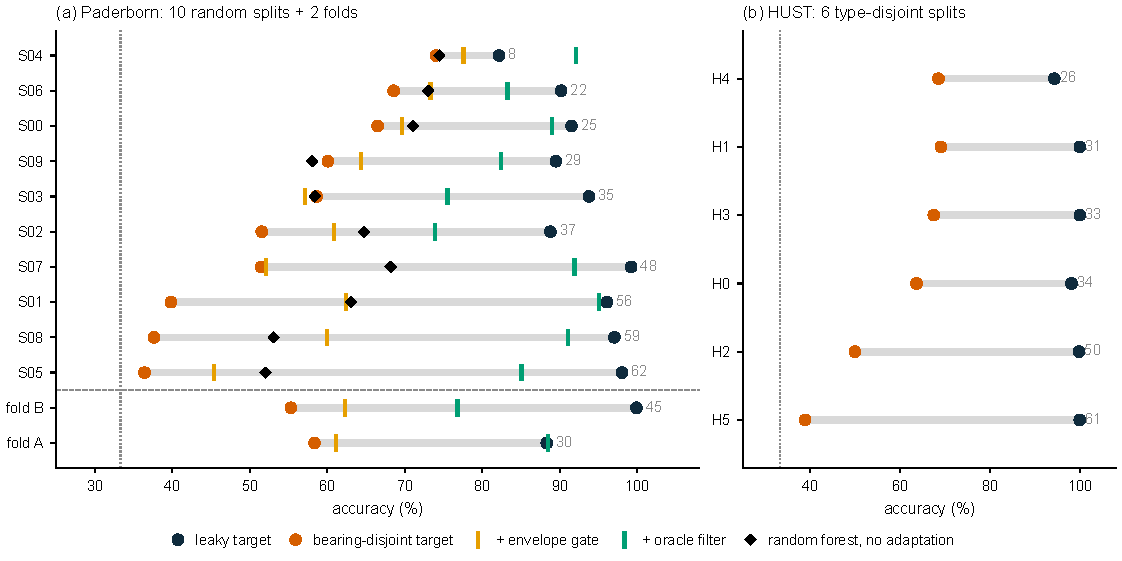
\includegraphics[width=\linewidth]{figures/fig2_collapse.pdf}
\caption{Accuracy by split on both rigs, rows sorted by the size of the collapse. Each row joins the leaky target (dark) to
the bearing-disjoint target (orange); ticks mark the same source model adapted with the envelope threshold gate (amber) and
with the oracle pseudo-label filter (green), and diamonds a random forest on ten time-domain statistics trained on the same
source windows without adaptation. The number at the right of each row is $\Delta_{\mathrm{leak}}$ in percentage points.
(a) Paderborn, ten pre-registered random bearing splits above the rule and the two mechanical folds below it (for the folds,
the ticks come from the gating job, whose source checkpoint differs from that of the dots; Section~\ref{sec:protocol});
(b) HUST bearing, six type-disjoint splits. Dotted line: three-class chance level.}
\label{fig:collapse}
\end{figure}

Across the ten pre-registered random splits (Table~\ref{tab:collapse}, Fig.~\ref{fig:collapse}) SDALR loses a median of 36.2
points on bearing-disjoint targets (95\,\% CI 25.0--56.3, range 8.2--61.6), positive in every split ($p=0.001$,
$p_{\mathrm{BH}}=0.002$). Which bearings happen to be in the source moves clean accuracy between \SI{36.4}{} and
\SI{74.0}{\percent}, which is why a single split --- the norm in this literature --- cannot support a performance claim. On
the two mechanical folds the leaky arm reaches \SI{94.1}{\percent} and the clean arm \SI{56.8}{\percent}, a loss of 30.0
points with fold~A as source and 44.6 with fold~B; with fold~B as source all six leaky tasks exceed \SI{99.7}{\percent} while
all six clean tasks fall between \SI{55.27}{} and \SI{55.33}{\percent}. The released checkpoint policy, which consults target
labels, gives \SI{94.7}{\percent} against \SI{57.8}{\percent} on the folds: target-label selection is worth 0.6 points on leaky
and 1.0 points on clean targets on average (per task 0.0--4.1), so it does not account for the gap.

\textbf{The gap is there before adaptation.} The batch-0 accuracy recorded in every adaptation log is the source model's
accuracy before any update. On the ten splits the source model alone already loses a median 35.1 points on unseen bearings
(CI 24.4--50.6, 10 of 10; Table~\ref{tab:collapse}, column ``Source-only $\Delta$''). SDALR's adaptation then changes the gap
by a median $+4.7$ points (positive in 8 of 10, two-sided $p = 0.18$): it raises leaky accuracy by a median 2.0 points and
lowers clean accuracy in 7 of 10 splits (median $-2.3$). On the folds adaptation adds 3.4 and 2.2 points on clean targets,
which is why an earlier reading of the folds alone suggested that adaptation helps there. Adaptation neither creates the
gap nor repairs it; the paper's subject is therefore what source-free adaptation inherits from its source model.

\textbf{The same bearing, seen and unseen.} Leaky and clean targets hold different bearings, so $\Delta_{\mathrm{leak}}$ also
contains the difference in difficulty between two bearing sets. Across the ten splits every bearing is in the source in some
splits and in the clean target in others, so its accuracy when seen can be compared with its accuracy when unseen
(Table~\ref{tab:bearings}, Fig.~\ref{fig:bearings}a). The within-bearing difference has a median of 38.7 points over the 17
bearings (CI 9.5--62.5): positive for 14 and tied for 3 (the healthy K003, K004 and K006, recognised perfectly either way); none is
negative. By class the median is 2.9 points for healthy specimens, 62.5 for outer-race and 49.0 for inner-race ones. Two
outer-race bearings, KA16 and KA30, are never correctly classified by SDALR when unseen. The seen and unseen scores come from
different adaptation runs and bearings share splits, so this contrast is descriptive; it holds the specimen fixed, which
the leaky--clean contrast cannot.

\subsection{The loss is not specific to one method, rig or condition shift}
\label{sec:res-second}

\begin{table}[htbp]
\centering
\caption{The collapse is not specific to one method: two source-free methods and four non-adaptive random forests on Paderborn, leaky versus bearing-disjoint targets (accuracy, \%).}
\label{tab:methods}
\begin{tabular}{lrrr}
\toprule
Method & Leaky & Clean & $\Delta_{\mathrm{leak}}$ \\
\midrule
SDALR, as released (target-label checkpoint) & 94.7 & 57.8 & 36.9 \\
SDALR, final checkpoint & 94.1 & 56.8 & 37.3 \\
SHOT, final iterate & 87.2 & 65.1 & 22.1 \\
\midrule
Random forest, 10 time statistics & 88.8 & 63.6 & 25.2 \\
Random forest, 64 spectral bands & 93.2 & 52.6 & 40.6 \\
Random forest, envelope spectrum & 76.7 & 43.1 & 33.5 \\
Random forest, all three feature sets & 95.4 & 60.3 & 35.1 \\
\midrule
Source model only (before adaptation), ten splits & 90.5 & 54.7 & 35.8 \\
Random forest, 10 time statistics, ten splits & 87.0 & 63.6 & 23.4 \\
Random forest, all three feature sets, ten splits & 93.1 & 57.6 & 35.5 \\
Random forest, 13 kinematic envelope features, ten splits & 67.4 & 54.3 & 13.1 \\
SHOT, final iterate, 10 splits & 82.7 & 57.4 & 25.3 \\
\bottomrule
\end{tabular}
\begin{minipage}{\linewidth}\vspace{2pt}\footnotesize All rows above the second rule use the same windows, the same two mechanical folds and the same 12 paired tasks; the random forests use no adaptation and no target data. No $p$-value is quoted for them: the tasks of a fold share a source checkpoint, so the unit is the fold, and two clusters cannot reach below $p = 0.25$ (Section~\ref{sec:protocol}). The rows below the second rule are means over the ten pre-registered splits, where the split is the unit; the time-statistics and combined forests collapse in 10 of 10 splits (exact sign-flip $p = 0.001$, $p_{\mathrm{BH}} = 0.002$). Source model only: batch-0 accuracy of the SDALR/SHOT source checkpoint before any adaptation step (median $\Delta$ 35.1~pp). Kinematic forest: record-level, maxima of the normalised envelope spectrum at the specimen's own BPFO/BPFI harmonics and shaft orders (median $\Delta_{\mathrm{leak}}$ 8.4~pp). SHOT over 10 splits: median $\Delta_{\mathrm{leak}}$ 21.7~pp, positive in 10 of 10 (exact sign-flip $p = 0.001$, $p_{\mathrm{BH}} = 0.002$). Differences are computed before rounding.\end{minipage}
\end{table}


\begin{table}[htbp]
\centering
\caption{Second rig: SDALR on HUST bearing, six pre-registered type-disjoint splits (accuracy, \%). The source is three bearing types; the clean target is the other two at the target load.}
\label{tab:hust}
\begin{tabular}{llrrr}
\toprule
Split & Source bearings & Leaky & Clean & $\Delta_{\mathrm{leak}}$ \\
\midrule
H0 & 6204, 6207, 6208 & 98.1 & 63.7 & 34.5 \\
H1 & 6204, 6205, 6207 & 100.0 & 69.1 & 30.9 \\
H2 & 6204, 6205, 6206 & 99.8 & 49.9 & 49.9 \\
H3 & 6205, 6206, 6207 & 100.0 & 67.5 & 32.5 \\
H4 & 6206, 6207, 6208 & 94.3 & 68.5 & 25.8 \\
H5 & 6205, 6206, 6208 & 100.0 & 38.9 & 61.1 \\
\bottomrule
\end{tabular}
\begin{minipage}{\linewidth}\vspace{2pt}\footnotesize Median $\Delta_{\mathrm{leak}}$ 33.5~pp (range 25.8--61.1, one-sided Wilcoxon $p=0.016$ over the six splits, which is the smallest value attainable with six clusters; exact sign-flip $p=0.016$, $p_{\mathrm{BH}}=0.022$, but $p_{\mathrm{BY}}=0.065$ under arbitrary dependence), which meets the replication rule fixed before the run. On this rig the clean target changes bearing size as well as bearing identity, so the shift is stronger than Paderborn's.\end{minipage}
\end{table}


Table~\ref{tab:methods} repeats the design for a second source-free method and for non-adaptive baselines. SHOT, in our
implementation and from the same source checkpoint, loses 22.1 points on the folds and a median of 21.7 over the ten splits
(CI 10.9--37.7, 10 of 10, $p = 0.001$, $p_{\mathrm{BH}} = 0.002$; the pre-registered rule --- a median loss of at least 10
points at $p < 0.05$ --- is met). Its smaller loss than SDALR's does not mean it transfers better: SHOT starts from the same
35.1-point source gap and narrows it mainly by lowering leaky accuracy (median $-5.3$ points) rather than by raising clean
accuracy (median $+3.7$). Random forests \cite{pedregosa2011sklearn} trained on the same source windows with no adaptation at all lose a median 22.7
points on ten time-domain statistics (CI 16.4--32.5) and 32.1 points on the combined feature set (CI 25.5--43.3), each in 10
of 10 splits ($p_{\mathrm{BH}} = 0.002$ each). On bearing-disjoint targets the time-statistics forest is more accurate than
adapted SDALR by a median 8.9 points (CI 0.4--16.1, 8 of 10 splits).

The result replicates on a second rig. On HUST bearing (Table~\ref{tab:hust}, Fig.~\ref{fig:collapse}b) mean leaky accuracy
is \SI{98.7}{\percent} and mean clean accuracy \SI{59.6}{\percent}, a median split-level loss of 33.5 points (CI 28.4--55.5,
$p=0.016$), meeting the replication rule fixed before the run. Each HUST bearing type is a different size, so the clean target
changes geometry as well as specimen, and with six clusters the result survives Benjamini--Hochberg but not
Benjamini--Yekutieli; it replicates direction and size.

\textbf{Without any condition shift.} Every task above crosses operating conditions. In a pre-registered control the time-
statistics forest is trained, at each condition separately, on half of the source bearings' recordings and tested at the
\emph{same} condition on the held-out recordings of the same bearings and on recordings of the complementary bearings;
recordings never cross the split, which is the separation used by recording-level benchmarks \cite{knap2026leakagesafe} and
the repetition-wise split of Vieira et al.\ \cite{vieira2026}. Balanced accuracy falls by a median of 29.7 points (CI
18.7--40.5, 10 of 10, $p_{\mathrm{BH}} = 0.002$), from a median \SI{94}{\percent} on held-out recordings of seen bearings to
\SI{65}{\percent} on unseen ones. Unseen-bearing accuracy is comparable with and without a condition shift (median balanced accuracy
\SI{65}{\percent} here, mean accuracy \SI{63.6}{\percent} across conditions), so condition shift is not what the leaky--clean
difference mainly measures. A post-hoc breakdown by class
locates the loss: healthy recall barely moves (median 99.9 to \SI{98.2}{\percent}); inner-race recall, where every bearing
carries the same mechanism (fatigue pitting \cite{lessmeier2016}), falls by a median 28.5 points; outer-race recall, which
mixes pitting with plastic deformation from indentations, falls by 66 points, and on unseen indentation bearings it is a
median \SI{23}{\percent} against \SI{64}{\percent} on pitting ones (medians over the ten and eight target sets that contain such bearings, folds included). This
control uses a forest; SDALR and SHOT were not run at a fixed condition.

\subsection{Why unseen bearings fail}
\label{sec:res-mechanism}

\begin{table}[htbp]
\centering
\caption{Per-bearing view of the Paderborn real-damage specimens: what each one is, how SDALR scores it when it was and was not in the source, and how often the envelope gate certifies it.}
\label{tab:bearings}
\small
\setlength{\tabcolsep}{4pt}
\begin{tabular}{lllllrrrr}
\toprule
Bearing & Mfr. & Damage & Extent & Size (mm) & Seen & Unseen & Diff. & Gate \\
\midrule
KA04 & FAG & pitting & 1 & 2 $\times$ 3 & 87 & 25 & +62 & 41/60 \\
KA15 & FAG & indentation & 1 & $<$1 $\times$ $<$1 & 68 & 29 & +39 & 0/60 \\
KA16 & MTK & pitting & 2 & 2 $\times$ full & 75 & 0 & +75 & 40/60 \\
KA22 & IBU/IBB & pitting & 1 & $<$2 $\times$ 1 & 100 & 55 & +45 & 0/60 \\
KA30 & MTK & indentation & 1 & $<$1 $\times$ $<$1 & 94 & 0 & +94 & 1/60 \\
KI04 & MTK & pitting & 1 & 2 $\times$ 1 & 84 & 61 & +23 & 0/60 \\
KI14 & MTK & pitting & 1 & 1 $\times$ 1 & 87 & 43 & +44 & 0/60 \\
KI16 & FAG & pitting & 3 & 6 $\times$ full & 95 & 41 & +54 & 32/60 \\
KI17 & MTK & pitting & 1 & 1 $\times$ 2 & 96 & 21 & +75 & 0/60 \\
KI18 & MTK & pitting & 2 & 2.5 $\times$ full & 96 & 31 & +65 & 45/60 \\
KI21 & FAG & pitting & 1 & 1 $\times$ 2 & 100 & 74 & +26 & 0/60 \\
\midrule
K001--K006 & IBU & healthy & -- & -- & 100 & 95 & +5 & 1/360$^{b}$ \\
\bottomrule
\end{tabular}
\begin{minipage}{\linewidth}\vspace{2pt}\footnotesize Manufacturer (page~1), damage mode, extent class (1--3) and damage length $\times$ width in mm (page~2) are read from each bearing's own Paderborn datasheet; pitting = fatigue pitting, indentation = particle-caused plastic deformation. Seen / unseen: SDALR window accuracy (\%) on that bearing over the ten splits in which it was in the source (scored in the leaky arm) or in the clean target. Gate: correct fault verdicts of the envelope threshold rule at the three adaptation conditions. $^{b}$ False acceptances. Over all 17 bearings the within-bearing difference has median 38.7~pp (95\,\% CI 9.5--62.5): 14 positive, 3 ties, 0 negative.\end{minipage}
\end{table}


\begin{figure}[htbp]
\centering
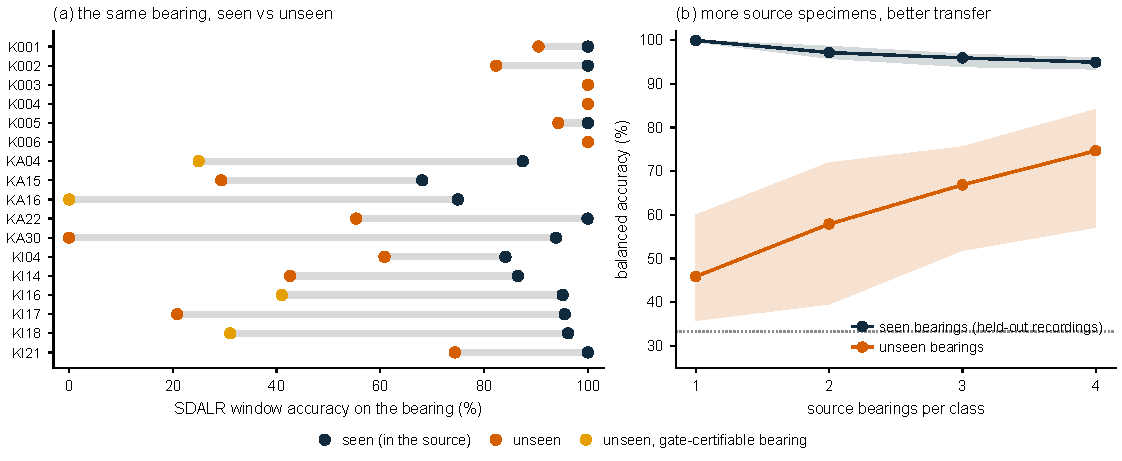
\includegraphics[width=\linewidth]{figures/fig3_bearings.pdf}
\caption{(a) SDALR accuracy on each Paderborn bearing over the ten splits, when it was in the source (dark) and when it was
unseen (orange; amber for the four bearings the envelope gate can certify). (b) Pre-registered source-diversity curve: a
random forest on ten time statistics, same-condition design, balanced accuracy on held-out recordings of the training
bearings (dark) and on one unseen bearing per class (orange), median and interquartile range over 30 test triples.}
\label{fig:bearings}
\end{figure}

Two explanations predict the same collapse. In one, a source-trained model learns to recognise its training specimens ---
a fixed identity shortcut --- and nothing about a new specimen. In the other, three specimens per class sample too little of
the variation in damage signatures (extent, shape, mechanism, manufacturer) for any classifier to cover a new one. The two
differ in what more source specimens would do, and in what a representation that encodes fault kinematics would do.

\textbf{Specimens are identifiable, but identifiability is not the failure.} A logistic-regression probe fitted within each
class on record-disjoint halves identifies the physical bearing in 507 of 508 held-out recordings from the frozen SDALR source
features and in 508 of 508 from ten elementary time statistics (pooled chance 0.35); the 508 recordings are the held-out half
of the 1020 source recordings of the six source models. The identification survives removing the signal mean, the statistic
most tied to sensor offset (508 of 508); the standard deviation alone identifies 477. It is not within-session drift: the
same probe asked to separate the first ten from the last ten recordings of one bearing succeeds on 285 of 508 (chance 254).
But healthy specimens are identified as perfectly as faulty ones (180 of 180) and still transfer (Table~\ref{tab:bearings}).
Identity is available in these signals; whether a classifier relies on it is a different question.

\textbf{More source specimens transfer better.} In a pre-registered curve the forest was trained on one to four source
bearings per class and tested on a fixed unseen bearing per class, for 30 test triples at each of the three conditions
(Fig.~\ref{fig:bearings}b). Balanced accuracy on the unseen bearings rises from a median \SI{45.9}{\percent} with one
specimen per class to 57.9, 66.9 and \SI{74.6}{\percent} with two, three and four, while accuracy on held-out recordings of
the training bearings stays at 95--100\,\%. The paired gain from one to four specimens has a median of 15.4 points over the
triples (25 of 30 positive, $p < 10^{-5}$), meeting the rule fixed before the run. A pure identity shortcut predicts a flat
curve; the measured one is steep. The collapse is therefore mainly under-sampling: with three specimens per class, the
source does not span the damage signatures it will meet, which is the supervised finding of Vieira et al.\ on the number of
training bearings \cite{vieira2026}, here measured as a curve under a fixed test set.

\textbf{Labelling whole specimens is not a sign of failure.} An adapted model that misclassifies an unseen bearing usually
does so for all its windows: with fold~B as source every clean bearing receives a single label across all six tasks, and the
resulting \SI{55.33}{\percent} is exact arithmetic (three healthy and two fault bearings right, $(2\,000 + 660 + 660)/6\,000$).
But block labelling is equally common when the bearing was seen: per task, \SI{90}{\percent} of seen and \SI{89}{\percent} of
unseen bearing--task pairs receive one label for at least \SI{99}{\percent} of their windows, and the fold~A direction is not
pure (K004 0.67, KI17 0.56). A specimen's windows are similar to each other, so a classifier decides the specimen as a whole;
the failure is in which label it gives, not in how it gives it.

\textbf{A kinematic representation leaks less but knows less.} The networks and forests above see 2048-sample windows,
which cannot represent the kinematic signature (Section~\ref{sec:windows}). A pre-registered forest on 13 kinematic features
of each full recording --- the floor-normalised envelope spectrum at the specimen's own first five outer- and inner-race
harmonics and at shaft orders 1--3 --- loses a median 8.4 points on unseen bearings (CI 4.8--21.0, 9 of 10 splits), below the
10-point threshold fixed in advance, so by its rule it transfers. Its accuracy is low on both arms (median \SI{65.8}{\percent}
leaky, \SI{56.1}{\percent} clean): the kinematic lines are visible only on the specimens with large damage (next subsection),
and a classifier that relies on them generalises as far as they are visible and no further. The representation decides how
much of what a model knows is specimen-specific; it does not by itself supply detectability. Concurrent work reports a
similar role for order-domain inputs in unsupervised adaptation across held-out Paderborn bearings, most of them with
artificial damage \cite{nagaswetha2026}.

\subsection{How much an oracle pseudo-label filter recovers}
\label{sec:res-decomp}

\begin{figure}[htbp]
\centering
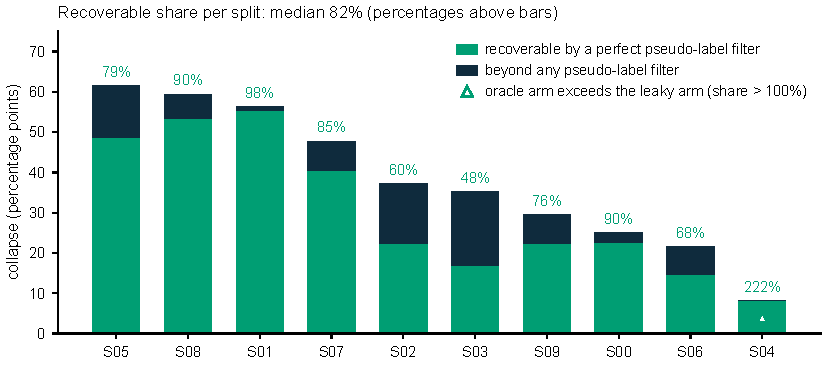
\includegraphics[width=\linewidth]{figures/fig4_decomposition.pdf}
\caption{Decomposition~\eqref{eq:decomp} per split: the part of the collapse an oracle pseudo-label filter recovers, and the
part it does not.}
\label{fig:decomp}
\end{figure}

On the ten random splits, where all four arms ran in one job, the oracle filter recovers a median \SI{82}{\percent} of the
collapse (CI 68--94, interquartile range 70--\SI{90}{\percent}, Fig.~\ref{fig:decomp}). The share varies: at
\SI{48}{\percent} on S03 half the collapse is not recovered, while on S04 --- the mildest collapse, 8.2 points --- the oracle
arm exceeds the leaky arm, a share of \SI{222}{\percent}. The fold-level decomposition is not reported, because the gating job
that produced the oracle arm has no leaky arm (Section~\ref{sec:protocol}).

The oracle withholds every incorrect pseudo-label and keeps every correct one; it is the keep-or-withhold counterpart of the
perfect-pseudo-label level of Schlachter et al.\ \cite{schlachter2025}. It is a reference for filters acting on this
method's pseudo-label step --- the family to which all four gates belong --- not a proven bound, and it says nothing about
methods that relabel, reweight continuously or change the representation. The part it does not recover mixes what the
source model carries with the difference in difficulty between the two bearing sets, as S04 shows. With that reading,
correct pseudo-labels alone would close most of the gap on this rig; the question for physics gating is how many of them it
can supply.

\subsection{Physics gating: safety, coverage and paired gains}
\label{sec:res-gating}

\begin{table}[htbp]
\centering
\caption{Gate safety on real healthy bearings. A false acceptance is a healthy recording given a fault verdict.}
\label{tab:gates}
\small
\setlength{\tabcolsep}{4pt}
\begin{tabular}{lrrrrr}
\toprule
Gate (swept parameter) & Op.\ point & Healthy FA & 95\,\% CI (\%) & Correct verdicts & At zero FA \\
\midrule
Envelope threshold rule (PCV-like), $z$ & 10 & 1/480 & 0.0--1.2 & 366 & 351 \\
Shaft-alias-guarded comb (comb\_v2), $\alpha$ & 0.05 & 0/480 & 0.0--0.8 & 312 & 312 \\
Surrogate-null comb test, $\alpha$ & 0.05 & 9/480 & 0.8--2.9 & 309 & -- \\
Raw-spectrum band rule (EAGLE-style), $z$ & 2 & 214/480 & 26.9--60.8 & 429 & 0 \\
\bottomrule
\end{tabular}
\begin{minipage}{\linewidth}\vspace{2pt}\footnotesize Population: 2{,}319 Paderborn recordings (480 healthy, 1{,}839 single inner- or outer-race). Operating points are the values fixed before the gates were evaluated. The last column sweeps each gate's parameter and reports the largest number of correct fault verdicts reachable while accepting no healthy recording. Intervals: bootstrap over the 6 healthy bearings where the count exceeds one, exact Clopper--Pearson over records otherwise. Full operating curves: Supplementary~S2. The population spans 29 physical bearings -- 6 healthy, 11 real-damage and 12 artificial-damage -- at all four operating conditions; coverage by damage origin is given in Section~\ref{sec:res-gating}.\end{minipage}
\end{table}


\begin{figure}[htbp]
\centering
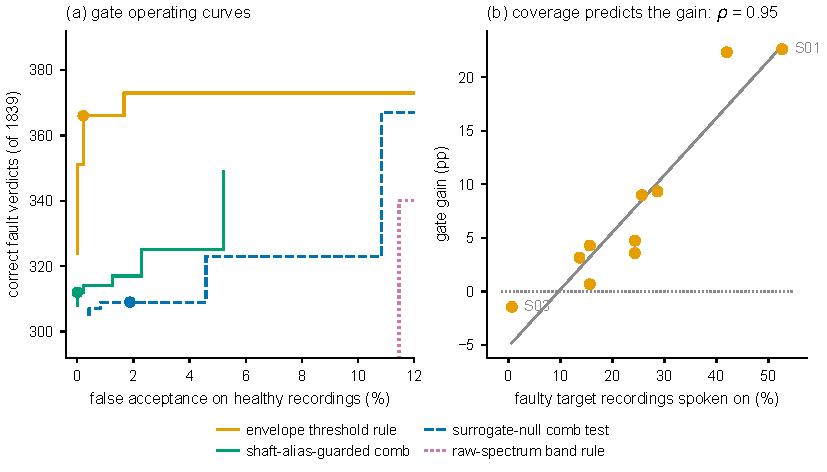
\includegraphics[width=\linewidth]{figures/fig5_roc.pdf}
\caption{(a) Gate operating curves on 2319 Paderborn recordings: correct fault verdicts against false acceptance on the 480
healthy recordings, as each gate's parameter is swept. Filled circles mark the operating points fixed before evaluation. The
vertical axis starts at 292 verdicts: the raw-spectrum band rule returns no correct verdict below \SI{11.5}{\percent} false
acceptance, and its operating point lies at \SI{45}{\percent}, off the right of the axis. (b) Per split ($n=10$), the share of
the clean target's faulty recordings the envelope gate gives a fault verdict against its paired accuracy gain. Spearman
$\rho = 0.95$; with the label-free share of all target recordings, $\rho = 0.93$. The line is a least-squares fit for reading
only.}
\label{fig:roc}
\end{figure}

\textbf{Safety.} Gate behaviour is characterised on all 2319 single-fault and healthy Paderborn recordings: 29 physical
bearings (6 healthy, 11 real-damage, 12 artificial-damage) at four operating conditions. At the operating points fixed
before evaluation (Table~\ref{tab:gates}) the envelope threshold rule accepts a fault on 1 of 480 healthy recordings (95\,\%
CI 0.0--1.2\,\%), the alias-guarded comb on none (0.0--0.8\,\%), the surrogate-null comb on 9 (0.8--2.9\,\%), and the
raw-spectrum band rule on 214 (26.9--60.8\,\%, bootstrapped over the six healthy bearings). Sweeping each gate's parameter
(Fig.~\ref{fig:roc}a) shows that this is not a threshold artefact: the envelope rule dominates at every false-acceptance
level and the raw-spectrum rule is dominated everywhere.

\textbf{Coverage, and what limits it.} No gate exceeds about \SI{20}{\percent} correct fault verdicts (the envelope rule's 373
of 1839) before false acceptance passes \SI{10}{\percent}. The comb tests, which add cepstral pre-whitening and a
record-specific null to the same kurtogram band selection, reach 323--349 below \SI{10}{\percent} false acceptance,
so the limit is not one detector's
design. Table~\ref{tab:bearings} shows where it lies. At the three adaptation conditions the envelope rule certifies 4 of the
11 real-damage bearings on more than one recording --- KA04 (41 of 60), KA16 (40), KI16 (32) and KI18 (45) --- and these are the
specimens with the largest damage: extent class 2 or 3, or a pit \SI{2}{mm} long and \SI{3}{mm} wide (KA04), with the damage
spanning the full raceway width on three of them. Every bearing it does not certify has extent class 1 and damage no larger
than \SI{2}{mm} in either dimension. The two comb tests certify the same four bearings (both also fire on a few recordings of
KI04, all wrongly, and of KA30); the raw-spectrum rule fires on every recording of those four, but also on bearings with no
envelope signature and on healthy ones. On this rig, envelope detectability is a
property of damage size, and a gate can only supply labels for the specimens whose damage is large enough to be seen.

\textbf{Inside the adaptation loop.} Over the ten splits the envelope gate adds a median 4.5 points to bearing-disjoint
accuracy (CI 2.5--15.7, positive in 9 of 10, $p=0.003$, $p_{\mathrm{BH}}=0.005$) and closes a median \SI{19}{\percent} of the
oracle gap (CI 10--41). Where it acts it changes what the model says --- with fold~B as source, KA04 moves from
\SI{100}{\percent} inner-race predictions to 71/29 inner/outer --- but the gain lies almost entirely on the recordings it
certifies (Table~\ref{tab:gateacc}). Splitting each split's clean windows by gate verdict, certified windows gain a median 47 points, uncovered faulty
windows a median 0.3 (sum over splits slightly negative) and healthy windows a median 0; certified windows carry
\SI{104}{\percent} of the summed gain. Because SFDA is scored on the windows it adapts on, a gain on certified windows is
partly the gate's own label returned. The size of the gain therefore follows coverage closely: across the splits it tracks
the share of faulty target recordings the gate speaks on ($\rho = 0.95$) and the label-free share of all target recordings
it speaks on ($\rho = 0.93$, $p = 10^{-4}$), and the latter survives partialling out headroom (oracle minus ungated clean;
partial $\rho = 0.90$, $p = 9\times10^{-4}$), whereas headroom given faulty-recording coverage predicts nothing (partial $\rho = 0.04$). The
coverage of a split is set by whether KA04, KA16, KI16 or KI18 are among its clean bearings. On S03, where the gate speaks
on two recordings of KA30 and is right on one, gating costs 1.5 points.

On the two mechanical folds, over three seeds, the alias-guarded comb adds a mean $+4.03$ points and the envelope rule
$+7.05$, positive in every seed (Table~\ref{tab:gains}, Fig.~\ref{fig:gains}); the comb was never run on the splits and no
general claim is made for it. The raw-spectrum band rule, run on the folds with one seed only, has a mean effect of $-3.9$
points that hides $+5.4$ with fold~A as source and $-13.2$ with fold~B: it injects confident wrong labels on healthy and
uncertified bearings, and whether that helps or hurts depends on which bearings are in the target.

\begin{table}[htbp]
\centering
\caption{Where the envelope-gate gain comes from: clean-target accuracy (\%) on certified and silent recordings.}
\label{tab:gateacc}
\small
\setlength{\tabcolsep}{4pt}
\begin{tabular}{lrrrrrrr}
\toprule
Split & Cert.\ (\%) & Certified & Silent faulty & Silent healthy & Gain & from cert. & from silent \\
\midrule
S00 & 12 & 51.2 $\to$ 99.2 & 59.5 $\to$ 55.2 & 83.5 $\to$ 83.5 & +3.1 & +5.6 & -2.4 \\
S01 & 37 & 10.1 $\to$ 70.3 & 9.3 $\to$ 11.2 & 100.0 $\to$ 100.0 & +22.6 & +22.0 & +0.6 \\
S02 & 20 & 29.8 $\to$ 75.8 & 26.3 $\to$ 27.0 & 100.0 $\to$ 100.0 & +9.3 & +9.0 & +0.3 \\
S03 & 1 & 0.0 $\to$ 0.5 & 38.4 $\to$ 36.2 & 99.7 $\to$ 99.7 & -1.5 & +0.0 & -1.5 \\
S04 & 17 & 50.5 $\to$ 71.0 & 64.8 $\to$ 64.8 & 100.0 $\to$ 100.0 & +3.6 & +3.6 & +0.0 \\
S05 & 14 & 4.3 $\to$ 55.7 & 22.8 $\to$ 22.8 & 71.9 $\to$ 76.7 & +9.0 & +7.3 & +1.6 \\
S06 & 17 & 49.2 $\to$ 74.1 & 54.1 $\to$ 55.0 & 100.0 $\to$ 100.0 & +4.7 & +4.3 & +0.4 \\
S07 & 9 & 38.6 $\to$ 55.8 & 29.5 $\to$ 30.6 & 93.3 $\to$ 88.7 & +0.7 & +1.5 & -0.9 \\
S08 & 31 & 10.0 $\to$ 80.4 & 3.5 $\to$ 5.3 & 100.0 $\to$ 100.0 & +22.3 & +21.7 & +0.7 \\
S09 & 9 & 7.4 $\to$ 76.6 & 45.1 $\to$ 42.0 & 100.0 $\to$ 100.0 & +4.3 & +6.1 & -1.8 \\
\bottomrule
\end{tabular}
\begin{minipage}{\linewidth}\vspace{2pt}\footnotesize Clean target of each split, SDALR ungated $\to$ with the envelope threshold gate, windows grouped by the gate verdict of their recording. Certified: a fault verdict; silent faulty and silent healthy: no verdict. The split's gain is the sum of the last two columns (group share $\times$ within-group change). Over the ten splits, certified windows gain a median 47~pp, silent faulty windows +0.3~pp; certified windows carry 104\,\% of the summed gain. SFDA is scored on the windows it adapts on, so the certified column partly returns the gate's own labels (C107).\end{minipage}
\end{table}


\begin{table}[htbp]
\centering
\caption{Paired per-task effect of gating inside SDALR on the 12 bearing-disjoint tasks of the two mechanical folds (gated $-$ ungated, percentage points).}
\label{tab:gains}
\small
\setlength{\tabcolsep}{4pt}
\begin{tabular}{llrrrrr}
\toprule
Gate & Seed & Mean & Median & Min & Max & Tasks $>0$ \\
\midrule
Shaft-alias-guarded comb & 0 & +3.79 & +3.33 & -0.08 & +11.01 & 7/12 \\
 & 1 & +4.56 & +3.28 & -0.08 & +15.45 & 8/12 \\
 & 2024 & +3.73 & +3.67 & -0.05 & +8.07 & 8/12 \\
\midrule
Envelope threshold rule & 0 & +7.44 & +7.57 & -0.01 & +18.02 & 9/12 \\
 & 1 & +7.99 & +6.65 & -0.70 & +19.44 & 10/12 \\
 & 2024 & +5.70 & +5.59 & -0.05 & +14.52 & 10/12 \\
\midrule
Raw-spectrum band rule & 2024 & -3.93 & -4.03 & -20.01 & +6.63 & 6/12 \\
\bottomrule
\end{tabular}
\begin{minipage}{\linewidth}\vspace{2pt}\footnotesize Every arm of a comparison runs in one job on the same source checkpoint, verified from identical pre-update target accuracy in each adaptation log, so these are paired differences. The between-seed spread of the per-task gain is 1.7~pp (comb) and 2.4~pp (envelope), against 2.8~pp for ungated per-task accuracy. No $p$-value is quoted: the 12 tasks of a seed come from two source folds, so the unit is the fold and two clusters cannot reach below $p = 0.25$. The inferential test is the ten-split comparison in Table~\ref{tab:collapse}. Raw-spectrum band rule: seed 2024 only and never run on the ten splits; its fold means are +5.35 (fold A source) and -13.21~pp (fold B source).\end{minipage}
\end{table}


\begin{figure}[htbp]
\centering
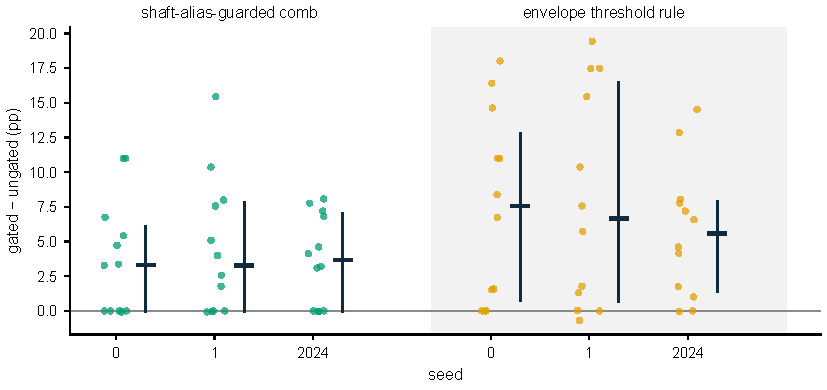
\includegraphics[width=\linewidth]{figures/fig6_gains.pdf}
\caption{Paired per-task effect of inserting each safe gate into the adaptation loop on the two folds, over three seeds.
Each point is one task; positive values are gains over the ungated arm trained from the same source checkpoint in the same
job. Horizontal mark: median; vertical bar: percentile bootstrap interval of the median over the 12 tasks (descriptive; tasks
of a fold share a checkpoint).}
\label{fig:gains}
\end{figure}

\textbf{Does the operating point need the target rig?} Gate verdicts use no target labels, but the evidence that $z = 10$ is
\emph{safe} comes from Paderborn's own healthy recordings, which is target-rig supervision. Swept on 24 healthy recordings
from two rigs that appear nowhere in the adaptation experiments --- 20 from UORED and 4 CWRU baselines, truncated to
Paderborn's spectral resolution --- the same rule needs $z = 36$ for zero false acceptance and accepts 4 of the 24 at $z = 10$.
On Paderborn the nearest swept point, $z = 40$, certifies 333 of 1839 fault recordings against 366 at $z = 10$
(\SI{91}{\percent} of the verdicts) with no healthy false acceptance. An operating point does not transfer between rigs and must be characterised on healthy recordings wherever the
gate is deployed; the adaptation arms were run at $z = 10$ only.

\section{Discussion}
\label{sec:discussion}

\paragraph{The error is in the source model, and both adaptation methods inherit it.} The gap between seen and unseen
bearings is present in the source model before any adaptation step (median 35.1 points) and is of the same size afterwards.
SDALR's self-training leaves it essentially unchanged; SHOT narrows it, but by giving up accuracy on the seen bearings rather
than by gaining on the unseen ones; a forest that never adapts shows it too. A source-free method can only refine what its
source model already separates, and on an unseen specimen the source model separates the wrong thing. This outcome was not
foregone. Self-training could have repaired the gap: the oracle arm shows that the same network, adapted with correct
pseudo-labels, recovers a median 82\,\% of it, so the network can be steered to most of the missing accuracy. The two methods' own
pseudo-labels simply carry the source model's errors forward. The question an
SFDA result on a bearing rig has to answer is therefore not ``how much does adaptation gain?'' but ``what did the source model
learn that transfers to a specimen it has not seen?''.

\paragraph{Under-sampling, not a fixed identity shortcut.} Individual specimens are identifiable from ten time statistics,
but that alone explains little: healthy specimens are identifiable too and transfer almost perfectly, and adding source
specimens raises a forest's unseen-bearing accuracy from 46 to 75\,\% with the test set fixed. Faulty specimens differ from each other in
what matters for the label --- the size, shape and mechanism of their damage (Table~\ref{tab:bearings}) --- and three of them per
class do not span that variation. This reading has a practical consequence the identity reading lacks: the remedy is more
diverse source specimens, as Vieira et al.\ found for supervised models \cite{vieira2026}, rather than an adversary that hides
specimen identity. A class-conditional identity adversary may still help at the margin, but the curve says diversity is where
most of the missing accuracy lies. The two readings are not exclusive: with one or two specimens per class, features
particular to those specimens separate the classes as well as any shared fault feature, and only a more diverse source makes
the shared features the cheaper solution. In that sense source diversity breaks the reliance on specimen-specific features;
the curve shows how much accuracy that is worth. The curve was measured with a forest; whether SDALR or SHOT follow it is
not measured.

\paragraph{Physics gating is bounded by detectability.} The safe gates help, consistently and modestly: a median 4.5 points
over the ten splits, essentially never costing anything. Three limits follow from the measurements. First, a filter can only
act through correct labels on the recordings it certifies, and the gain lies almost entirely there; the gate does not teach
the model anything that carries over to recordings it is silent on. Second, the envelope gates certify only the specimens with
the largest damage, and every envelope-based gate we tried certifies the same ones; detectability is a property of the damage, not of
the threshold. Third, an oracle filter shows that correct pseudo-labels on every recording would recover most of the gap, so
the room is there --- but it is room that envelope evidence cannot fill for small, early-stage damage, which is the damage a
monitoring system most needs to detect. A kinematic representation leaks less for the same reason: it relies only on what is
visible, and on this rig that is the large damage.

\paragraph{Safety is a property to measure, not to assume.} The raw-spectrum band rule accepts \SI{45}{\percent} of healthy
recordings as faulty; the envelope rules accept at most \SI{2}{\percent}. Inside the loop the safe gates never cost more than
1.5 points on a split, whereas the unsafe rule moved accuracy by $+5.4$ or $-13.2$ points depending on which bearings were in
the target. A module that injects confident wrong labels can look helpful on one target and harmful on another, and end
accuracy on one leaky protocol cannot tell a safe prior from an unsafe one. False acceptance on healthy recordings can.

\paragraph{A shallow baseline belongs in every such comparison.} On bearing-disjoint targets a forest on ten time-domain
statistics --- no adaptation, no target data, no deep network --- is more accurate than adapted SDALR in 8 of 10 splits. It is
not a better diagnostic method; it collapses too. It is a calibration point that any claim of transferable fault structure
should clear.

\paragraph{Is this leakage, or a different task?} Adapting to the same physical bearings at a new operating condition is a
legitimate task for a permanently instrumented asset. Two scenarios are conflated in the current literature. In the first the
monitored bearing is present in training, and same-bearing evaluation estimates performance honestly. In the second ---
a replacement bearing, a sister machine, a fleet --- the specimen at test time was never seen, and same-bearing evaluation
over-estimates performance by 22--36 points (median over splits, across the methods measured here). The problem is not the
published protocol in itself but reading its number as evidence for the second scenario. We use ``leakage'' in the sense of
Kapoor and Narayanan \cite{kapoor2023leakage}: information shared between training and evaluation that inflates the estimate
relative to the deployment the claim addresses.

\paragraph{Threats to validity.} The leaky and clean targets differ in their bearing sets; the within-bearing contrast holds
the specimen fixed and gives the same answer. The splits share bearings from a pool of 17, so their $p$-values are conditional
on this pool. The two folds are asymmetric (fold~B has two outer-race source bearings) and ran in two jobs with different
source checkpoints, which is why the folds are descriptive. The HUST replication changes bearing size along with the
specimen. Finally, the windows given to the networks cannot carry the kinematic signature; the kinematic-feature forest shows
what changes when the input can.

\section{What a source-free bearing-diagnosis result should carry}
\label{sec:recommendations}

The measurements above suggest eight pieces of evidence that separate a transferable result from a leaky one. None requires
new hardware; together they cost a few additional runs.

\begin{enumerate}
  \item \textbf{Bearing-disjoint targets.} Report accuracy on physical bearings absent from source training. If the dataset
        cannot support this --- CWRU's healthy class is effectively one specimen --- say so, and treat the published number as
        an upper bound rather than an estimate.
  \item \textbf{A distribution over splits.} Which bearings fell in the source moved clean accuracy between \SI{36}{} and
        \SI{74}{\percent} here. Report medians with intervals over several pre-registered draws, and a within-bearing contrast
        where bearings rotate between source and target.
  \item \textbf{The source-only gap beside the adapted one.} The batch-0 accuracy is already in every adaptation log. Here it
        showed that adaptation neither created nor repaired the gap, which no adapted number alone can show.
  \item \textbf{Paired differences for any add-on module.} Gates, regularisers and losses should be compared against the
        base method trained from the \emph{same} source checkpoint in the same job, and reported as the distribution of
        per-task or per-split differences.
  \item \textbf{An oracle pseudo-label reference.} One extra run per configuration, replacing the pseudo-label rule by the
        true label, converts a bare gain into a share of what correct labels would achieve.
  \item \textbf{A non-adaptive shallow baseline under the identical split.} Here it beat the adapted method in 8 of 10
        splits.
  \item \textbf{False acceptance and coverage for any physics module, measured on healthy recordings from the target rig.}
        A gate that certifies faults on healthy machinery injects confident wrong labels; a gate that certifies almost
        nothing cannot help, and its gain should be reported separately on the recordings it certifies and on the rest.
        Characterising a gate on target-rig healthy recordings is target-rig supervision, mild but real, and should be
        declared; our operating point, safe on Paderborn, accepted 4 of 24 healthy recordings from two other rigs.
  \item \textbf{A statement of whether model selection saw target labels.} The released selection rule was worth 0.6 points
        on leaky and 1.0 on clean targets on average, and up to 4.1 on a single task; headline numbers should use a rule that
        touches no target label.
\end{enumerate}

For deployment the same list reads as a risk assessment. A diagnosis system validated only with the monitored bearing present
in training has not been validated for the bearing it will meet in service; the drop measured here was a median 22--36 points
across methods. The most effective lever we measured is the number of distinct specimens in the source: going from one to four
per class raised unseen-bearing accuracy by a median 15 points. Where a kinematic gate is available and its false acceptance
has been characterised on healthy machinery, it is a low-risk addition, but it supplies labels only for damage large enough to
be seen in the envelope spectrum.

\section{Limitations}
\label{sec:limitations}

The experiments concern cross-condition transfer with bearing-disjoint targets on two test rigs; no cross-machine claim is
made. Paderborn carries the full analysis; HUST only replicates the collapse, and its splits change bearing size together
with the specimen. HUST's unpublished pitch diameter keeps it out of every kinematic analysis.

Two source-free methods are evaluated, SDALR from its released code and SHOT in our implementation from the same source
checkpoint. Neighbourhood-based methods such as NRC \cite{yang2021nrc} and AaD \cite{yang2022aad} remain to be tested; since
the gap is already in the source model, we expect them to inherit it --- they refine neighbourhoods of the source representation, and on an unseen
specimen those neighbourhoods are the specimen's own windows, which are already labelled as a block --- but this is not
shown. Every statement about
source-free adaptation here is a statement about these two methods under this protocol. The networks use SDALR's 2048-sample
windows, which cannot represent the kinematic signature; a source-free method on order-domain inputs of full recordings was
not run, and only a forest tested that representation.

Seeds and splits are traded against each other: three seeds on the two folds and one seed on each of the ten random splits and
six HUST splits. The splits share bearings, so their cluster-level $p$-values assume an exchangeability that holds only
approximately and apply to draws from this pool of 17 bearings. The two folds ran in two jobs that trained different source
checkpoints; no reported comparison crosses them, and the fold-level oracle decomposition is withdrawn for that reason. The
analyses added in this revision --- source-only arm, within-bearing contrast, spillover, purity, intervals --- are post-hoc and
descriptive; the source-diversity curve and the kinematic-feature forest were pre-registered.

A bearing-disjoint split changes the damage along with the specimen. Of the five real outer-race bearings, KA04, KA16 and KA22
carry fatigue pitting while KA15 and KA30 carry particle-caused plastic deformation; all six real inner-race bearings carry
fatigue pitting (\cite{lessmeier2016}, Table~5, corresponding to ISO~15243 clauses 5.1 and 5.5 \cite{iso15243}). Damage extent
ranges from class 1 to 3 (Table~\ref{tab:bearings}). Ten random splits average over this variation but do not remove it, and
each bearing was recorded in its own session and mounting, which no design here crosses. The same-condition control and the
source-diversity curve use a forest on time statistics; SDALR and SHOT were not run at a fixed condition or with more source
specimens, so whether adaptation changes those results is not measured. The source-diversity curve can only reach four
specimens per class on a rig with five or six; whether accuracy keeps rising beyond that is open.

The gating results inherit the detectability of envelope analysis on these specimens: four of the eleven real-damage bearings
carry a visible signature at the adaptation conditions, ball faults are absent from the Paderborn real-damage label space, and
the raw-spectrum band rule is our implementation of a published description, not the authors' code; we never compare it with
the accuracy published for the method it comes from. A remedy that removes specimen identity from the source representation
was pre-registered but cut for budget before any outcome was observed; the source-diversity curve suggests that source
diversity is the larger lever.

\section{Conclusions}
\label{sec:conclusions}

The source-free adaptation results we tested do not survive evaluation on bearings the source model has never seen. On
Paderborn SDALR loses a median 36.2 points over ten pre-registered bearing splits, and a given bearing loses a median 38.7
points when it is unseen rather than seen; SHOT loses 21.7 points, non-adaptive forests 22.7--32.1, a forest at a fixed
operating condition 29.7, and SDALR on a second rig 33.5. Near-ceiling accuracy under the conventional protocol and roughly
\SI{55}{\percent} under a bearing-disjoint one are the same models measured two ways.

The loss is in the source model, and both adaptation methods inherit it. The source model alone already loses 35.1 points before any
adaptation step; SDALR leaves the gap unchanged and SHOT narrows it only by losing accuracy on the seen bearings. The cause is
mainly under-sampling rather than a fixed identity shortcut: specimens are identifiable from simple statistics, but
a forest's unseen-bearing accuracy rises from 46 to 75\,\% as the source grows from one to four specimens per class, because faulty
specimens differ in the size, shape and mechanism of their damage.

Physics gating is safe and bounded. Envelope-based kinematic gates accept 0 to 9 of 480 healthy recordings as faulty, against
214 for a raw-spectrum band rule, and add a median 4.5 points inside the adaptation loop, closing about a fifth of the gap that
an oracle pseudo-label filter closes. The gain lies on the recordings the gate certifies, and the gates certify only the
specimens with the largest damage; a classifier built on the same kinematic evidence leaks little but is no more accurate. On
this rig, what limits physics-gated adaptation is the detectability of small damage, not the gate.

For practice the implication is procedural: bearing-disjoint targets over several splits, the source-only gap beside the
adapted one, paired differences from a shared checkpoint, an oracle reference, a shallow baseline, measured false acceptance
and coverage for any physics module (which requires verified healthy recordings from the target machine), and a statement of whether model selection saw target labels. They cost a handful of
extra runs, and they are what separates a transferable diagnosis from one that knows only the bearings it was trained on.

\section*{CRediT authorship contribution statement}
\textbf{Mohammad Rafiur Rahman:} Conceptualization, Methodology, Software, Validation, Formal analysis, Investigation,
Data curation, Writing -- original draft, Writing -- review \& editing, Visualization, Project administration.

\section*{Declaration of competing interest}

The author declares no known competing financial interests or personal relationships that could have
appeared to influence the work reported in this paper.

\section*{Funding}
% Complete before submission, or state that no specific grant was received.
This research did not receive any specific grant from funding agencies in the public, commercial, or not-for-profit
sectors.

\section*{Data availability}

All raw data are public. Paderborn bearing data are distributed by the KAt-DataCenter, Universit\"at Paderborn
\cite{lessmeier2016}; HUST bearing is available from Mendeley Data (\url{https://doi.org/10.17632/cbv7jyx4p9})
\cite{thuan2023hust}; CWRU bearing data from the Case Western Reserve University Bearing Data Center \cite{smith2015};
UORED-VAFCLS from the University of Ottawa \cite{sehri2023uored}; and the JNU data are those of Li et al.\ \cite{li2013jnu}.
The research data produced in this study --- the frozen split definitions, the per-run experiment ledger (one row per run
and task, each with its kernel, commit and artifact path), the analysis scripts with their checksums, the version-controlled
protocol and the retained run artifacts that back every number in this paper --- are available at \url{https://github.com/rafilovestosuffer/physgate-sfda} and archived
with a DOI [Zenodo DOI to be added at release].

\section*{Code availability}

The evaluation protocol, gate implementations, analysis and figure scripts are released with the research data. SDALR is
run from its authors' released code (BdLab405/SDALR, commit fb9c379), which the repository fetches by script because
it carries no licence for redistribution; the evaluation wrapper and the gate hook described in Section~\ref{sec:protocol} are
added around it without changing its training code. SHOT is our implementation of the published template and is released
with the rest.

\section*{Declaration of generative AI and AI-assisted technologies in the manuscript preparation process}

During the preparation of this work the author used Claude (Anthropic; through the Claude Code agent, with the model
claude-opus-5-5 in the final revision) in order to draft and edit text, write analysis and figure code, draw the schematic
figures with plotting code, and check numerical consistency and references against the retained artifacts and primary
sources. After using this tool, the author reviewed and edited the content as needed and takes full responsibility for the
content of the publication. Because the same tool also executed analyses and compute jobs, that use forms part of the
research method and is described in Section~\ref{sec:protocol}.


\bibliographystyle{elsarticle-num}
\bibliography{references}

\end{document}
